% Source: ne630_problems/lesson_26 at 9c3dc61; student statements match HW26.md.

% Adapted solutions correct legacy units, arithmetic, and data inconsistencies.

\noindent{\bf Problem 1 [FNRP 5.4]}

Suppose that a fissile material is discovered for which all fission
neutrons are emitted promptly. A reactor fueled with this material has a
constant neutron lifetime \(l=0.002~\mathrm{s}\), and its neutron
population is governed by FNRP Eq. (5.22). Assume a fixed flux shape, so
fission power is proportional to neutron population. Neglect feedback.

The reactor is initially critical and has no external neutron source. At
\(t=0\), impose a step change in reactivity and hold the new value
constant.

\begin{itemize}
\setlength{\itemsep}{0pt}\setlength{\parskip}{0pt}
\item
  \textbf{(a)} What reactor period is required for the power to triple
  in \(10~\mathrm{s}\)?
\item
  \textbf{(b)} Determine the required multiplication factor \(k\) and
  reactivity \(\rho=(k-1)/k\). Express \(\rho\) as a dimensionless
  quantity and in pcm.
\end{itemize}

The reactor period is the time required for the neutron population to
increase by a factor of \(e\). One pcm is \(10^{-5}\) in dimensionless
reactivity.


\begin{adaptedsolution}
With no source and all neutrons prompt,
\[
\frac{dn}{dt}=\frac{k-1}{l}n,\qquad
\frac{P(t)}{P(0)}=\exp\!\left(\frac{k-1}{l}t\right)=e^{t/T_R}.
\]
\textbf{(a)} Tripling in 10 s requires
\[
\boxed{T_R=\frac{10}{\ln3}=9.10239~\mathrm{s}.}
\]
\textbf{(b)} Therefore
\[
\boxed{k=1+\frac{l}{T_R}=1.000219722,}
\qquad
\boxed{\rho=\frac{k-1}{k}=\frac{l}{T_R+l}
=2.19674\times10^{-4}=21.9674~\mathrm{pcm}.}
\]
The specified $l$ is neutron lifetime. The generation time is $\Lambda=l/k$, so the equivalent exponent is $\rho/\Lambda$, not exactly $\rho/l$. Substitution into the exponential recovers $P(10)/P(0)=3$.
\end{adaptedsolution}

\newpage

\noindent{\bf Problem 2}

Consider the infinite, homogeneous water--uranium medium from Homework
13, Problem 2, but assume that all fission neutrons are prompt. The
two-group cross sections are repeated below; all are in
\(\mathrm{cm^{-1}}\).

\begin{longtable}[]{@{}lrr@{}}
\toprule\noalign{}
Quantity & Group 1 & Group 2 \\
\midrule\noalign{}
\endhead
\bottomrule\noalign{}
\endlastfoot
\(\Sigma_\gamma\) & \(2.04\times10^{-3}\) & \(1.91\times10^{-2}\) \\
\(\Sigma_f\) & \(2.96\times10^{-4}\) & \(1.38\times10^{-2}\) \\
\(\overline\nu\Sigma_f\) & \(7.38\times10^{-4}\) &
\(3.36\times10^{-2}\) \\
\(\Sigma_{s,1\gets g}\) & \(7.21\times10^{-1}\) & \(0\) \\
\(\Sigma_{s,2\gets g}\) & \(4.27\times10^{-2}\) & \(2.72\) \\
\end{longtable}

Use \(\Sigma_{a,g}=\Sigma_{\gamma,g}+\Sigma_{f,g}\) and mean group
speeds \(\bar v_1=10^6~\mathrm{m/s}\) and
\(\bar v_2=2.2\times10^3~\mathrm{m/s}\). For this one-group transient
approximation, assume a fixed spectrum with

\[
\frac{\phi_1(t)}{\phi_2(t)}
=\frac{\Sigma_{a,2}}{\Sigma_{s,2\gets1}}.
\]

This is the steady two-group spectral shape for fast-only fission and
external sources with no upscatter. Impose this shape throughout the
transient, rather than solving separate time-dependent group equations.

Initially the neutron population is zero. At \(t=0\), switch on a
uniform fast-neutron source of strength
\(S_0=100~\mathrm{neutrons\,cm^{-3}\,s^{-1}}\) and hold it constant.
Neglect changes in the material properties and feedback.

\begin{itemize}
\setlength{\itemsep}{0pt}\setlength{\parskip}{0pt}
\item
  \textbf{(a)} Determine the effective one-group absorption cross
  section \(\bar\Sigma_a\).
\item
  \textbf{(b)} Determine the mean neutron speed \(\bar v\). Be
  consistent about converting meters to centimeters.
\item
  \textbf{(c)} Determine the mean neutron lifetime \(l_\infty\).
\item
  \textbf{(d)} Collapse \(\overline\nu\Sigma_f\) with the same flux
  weights and determine \(k_\infty\) and \(\rho_\infty\) for the
  one-group model.
\item
  \textbf{(e)} Write and solve the initial-value problem for the total
  neutron number density \(n'''(t)\). Compute and plot the
  \textbf{volumetric absorption rate},
  \(R_a(t)=\bar\Sigma_a\bar v\,n'''(t)\), for
  \(0\le t\le0.1~\mathrm{s}\). Determine its steady limit and compare it
  with Homework 13, Problem 2. Explain why the steady limits agree even
  though a fixed spectrum is an approximation during the transient.
\end{itemize}


\begin{adaptedsolution}
The absorption cross sections and fixed flux ratio are
\[
\Sigma_{a,1}=0.002336,\quad\Sigma_{a,2}=0.0329~\mathrm{cm^{-1}},\qquad
r=\frac{\phi_1}{\phi_2}=\frac{0.0329}{0.0427}=0.770491803.
\]
Thus the flux weights are $w_1=r/(1+r)=0.435185185$ and
$w_2=1/(1+r)=0.564814815$.

\textbf{(a)} Flux-weighted collapse gives
\[
\boxed{\bar\Sigma_a=w_1\Sigma_{a,1}+w_2\Sigma_{a,2}
=0.019599~\mathrm{cm^{-1}}.}
\]
\textbf{(b)} Convert the speeds to $v_1=10^8$ and $v_2=2.2\times10^5~\mathrm{cm/s}$. As in Homework 25,
\[
\boxed{\bar v=\left(\frac{w_1}{v_1}+\frac{w_2}{v_2}\right)^{-1}
=3.88849\times10^5~\mathrm{cm/s}.}
\]
\textbf{(c)} The lifetime is
\[
\boxed{l_\infty=\frac{1}{\bar v\bar\Sigma_a}
=1.31215\times10^{-4}~\mathrm{s}.}
\]
\textbf{(d)} With the same flux weights,
\[
\overline{\nu\Sigma_f}=w_1(0.000738)+w_2(0.0336)
=0.0192989444~\mathrm{cm^{-1}},
\]
\[
\boxed{k_\infty=\frac{\overline{\nu\Sigma_f}}{\bar\Sigma_a}
=0.984690262,\qquad
\rho_\infty=\frac{k_\infty-1}{k_\infty}
=-0.0155477703=-1554.777~\mathrm{pcm}.}
\]
For this fixed shape the same $k_\infty$ follows from the two-group expression
\[
k_\infty=\frac{\nu\Sigma_{f,1}
+\nu\Sigma_{f,2}\Sigma_{s,2\gets1}/\Sigma_{a,2}}
{\Sigma_{a,1}+\Sigma_{s,2\gets1}}.
\]
Use $\Sigma_{s,2\gets1}=0.0427$ and the unrounded removal cross section
$\Sigma_{r,1}=0.045036~\mathrm{cm^{-1}}$ throughout. Using $0.0426$ in one calculation or rounding $\Sigma_{r,1}$ to $0.0450$ before subtraction spoils the comparison.

\textbf{(e)} The one-group initial-value problem is
\[
\frac{dn'''}{dt}=-\frac{1-k_\infty}{l_\infty}n'''+S_0,
\qquad n'''(0)=0.
\]
Define $\tau=l_\infty/(1-k_\infty)=0.00857071923~\mathrm{s}$. Then
\[
\boxed{n'''(t)=S_0\tau(1-e^{-t/\tau}),\qquad
R_a(t)=\frac{S_0}{1-k_\infty}(1-e^{-t/\tau}).}
\]
The steady limits are
\[
n'''(\infty)=0.857071923~\mathrm{cm^{-3}},\qquad
\boxed{R_a(\infty)=6531.79041~\mathrm{cm^{-3}\,s^{-1}}.}
\]
At $t=0.1~\mathrm{s}$, $R_a=6531.73445~\mathrm{cm^{-3}\,s^{-1}}$.
\begin{center}
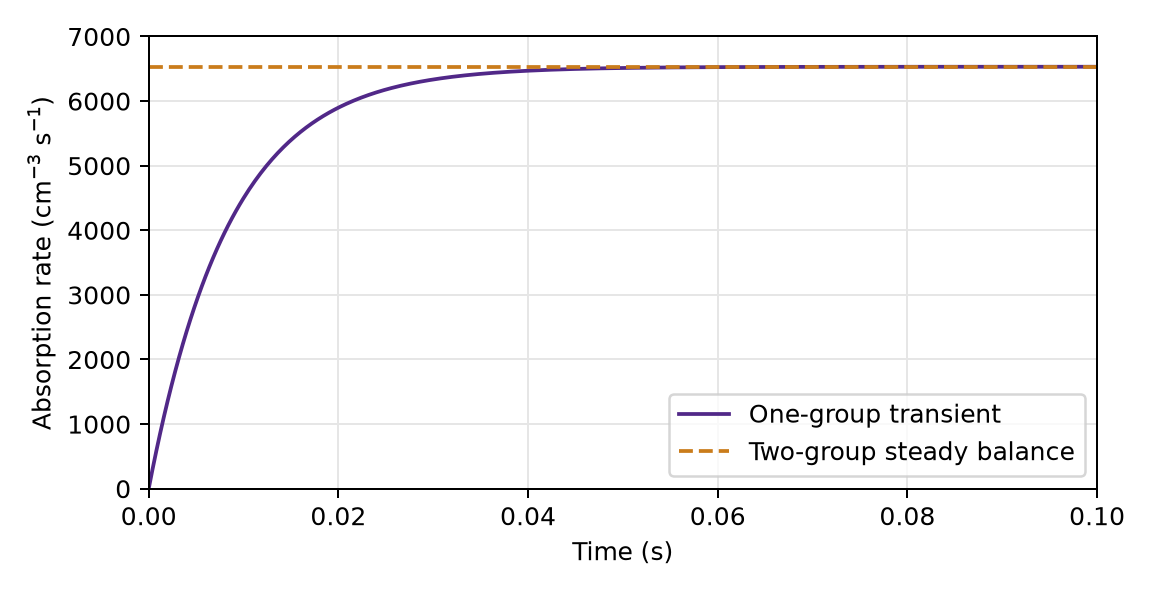
\includegraphics[width=.86\linewidth]{hw26_absorption_rate.png}
\end{center}
An independent steady two-group source calculation gives
\[
\phi_{1,\mathrm{ss}}=1.45034870\times10^5,\qquad
\phi_{2,\mathrm{ss}}=1.88236746\times10^5~\mathrm{cm^{-2}\,s^{-1}}.
\]
Hence $\Sigma_{a,1}\phi_{1,\mathrm{ss}}+\Sigma_{a,2}\phi_{2,\mathrm{ss}}$
recovers the same absorption rate as Homework 13 with these data. The imposed spectrum satisfies the exact steady thermal-group balance, so the steady limits agree. It need not describe the initially fast-only population: the full two-group transient generally has an evolving spectrum.
\end{adaptedsolution}

\newpage

\noindent{\bf Problem 3: Pulsed Accelerator-Driven Reactor}

Consider an idealized one-group accelerator-driven subcritical reactor
with

\[
k=0.95,\qquad l=10^{-4}~\mathrm{s},\qquad
\bar\nu=2.5,\qquad E_f=200~\mathrm{MeV/fission}.
\]

Here, \(E_f\) is recoverable fission energy. A proton accelerator sends
\textbf{1-GeV protons} to a neutron-producing target. The beam current
is \textbf{10 mA during each 1-ms pulse}, and pulses begin every
\textbf{10 ms}. The current is zero between pulses. Each incident proton
supplies \textbf{20 effective source neutrons} to the reactor; this
yield already includes target-to-core coupling. The accelerator draws
\textbf{25 MW of electrical power while the beam is on} and zero between
pulses.

Assume a fixed spatial shape and energy spectrum, constant reactor
properties, all fission neutrons emitted promptly, and negligible
feedback and depletion. Count only fission energy as reactor thermal
power; neglect direct beam heating. The parameters define a hypothetical
teaching model. Use \(e=1.602176634\times10^{-19}~\mathrm{C}\) and
\(1~\mathrm{eV}=1.602176634\times10^{-19}~\mathrm{J}\).

After many pulses, the neutron population is periodic:
\(n(t+T_c)=n(t)\), where \(T_c=10~\mathrm{ms}\) includes both the on-
and off-time. For any quantity \(X(t)\), define

\[
\langle X\rangle=\frac{1}{T_c}\int_0^{T_c}X(t)\,dt.
\]

\begin{itemize}
\item
  \textbf{(a)} Determine the duty factor, proton rate and neutron source
  strength during a pulse, and cycle-averaged neutron source strength.
  Also calculate the proton beam power while on and its cycle average.
  Distinguish beam power from the specified electrical consumption.
\item
  \textbf{(b)} Starting from

  \[
  \frac{dn}{dt}=\frac{k-1}{l}n(t)+S(t),
  \]

  integrate over one \textbf{complete cycle} to determine the average
  neutron population without solving the transient. Do not assume that
  \(n(t)\) is constant during the cycle or zero between pulses.
\item
  \textbf{(c)} The fission-neutron production rate is \(k n(t)/l\).
  Determine the cycle-averaged fission rate and reactor thermal power.
  Calculate the fission energy released per cycle and compare the
  average thermal power with the average accelerator electrical
  consumption. Explain why this comparison alone does not determine net
  electrical output.
\item
  \textbf{(d)} Predict how the average thermal power and electrical
  consumption change if the pulse duration doubles to \(2~\mathrm{ms}\)
  while the repetition period and peak current remain fixed. Then
  compare the original pulsed case with a continuous beam having the
  \textbf{same average current}. Does pulsing itself increase average
  reactor thermal power under these assumptions?
\end{itemize}

In this problem, \(n(t)\) is the total neutron population and \(S(t)\)
is the total source rate in neutrons/s, not a source density.


\begin{draftsolution}
\textbf{(a)} The duty factor is $D=T_{\rm on}/T_c=0.1$. During a pulse,
\[
\dot N_{p,\rm on}=\frac{I_{\rm on}}{e}
=\frac{0.010}{1.602176634\times10^{-19}}
=6.24150907\times10^{16}~\mathrm{s^{-1}},
\]
\[
S_{\rm on}=20\dot N_{p,\rm on}=1.24830181\times10^{18}~\mathrm{s^{-1}},
\qquad \boxed{\langle S\rangle=DS_{\rm on}=1.24830181\times10^{17}~\mathrm{s^{-1}}.}
\]
Each proton carries $1.602176634\times10^{-10}$ J, so
\[
P_{\rm beam,on}=10~\mathrm{MW},\qquad
\langle P_{\rm beam}\rangle=1~\mathrm{MW}.
\]
These are beam powers, not electrical consumption. The given 25-MW on-state draw corresponds to a 40\% beam-to-wall-plug efficiency.

\textbf{(b)} Integrating over a complete periodic cycle gives
\[
0=n(T_c)-n(0)=\frac{k-1}{l}T_c\langle n\rangle+T_c\langle S\rangle.
\]
Therefore
\[
\boxed{\langle n\rangle=\frac{l\langle S\rangle}{1-k}
=2.49660363\times10^{14}~\text{neutrons}.}
\]
No assumption of constant $n$ or instantaneous disappearance at beam shutoff is involved. The subcritical relaxation time is $\tau=l/(1-k)=2~\mathrm{ms}$.

\textbf{(c)} Divide fission-neutron production by $\bar\nu$ to get the fission rate:
\[
\boxed{\langle\dot F\rangle=\frac{k}{\bar\nu l}\langle n\rangle
=\frac{k\langle S\rangle}{\bar\nu(1-k)}
=9.48709379\times10^{17}~\mathrm{fissions/s}.}
\]
Using $E_f=3.204353268\times10^{-11}~\mathrm{J/fission}$,
\[
\boxed{\langle P_{\rm th}\rangle=E_f\langle\dot F\rangle=30.4~\mathrm{MW},\qquad
E_{\rm cycle}=\langle P_{\rm th}\rangle T_c=0.304~\mathrm{MJ}.}
\]
The mean electrical consumption is $\langle P_{\rm elec}\rangle=D(25)=2.5~\mathrm{MW}$, giving a thermal-to-accelerator-electric ratio of $30.4/2.5=12.16$.
This is not a net electrical gain. If $\eta_{\rm th\to e}$ is the thermal-to-electric efficiency and other loads are neglected,
$\langle P_{\rm net,e}\rangle=\eta_{\rm th\to e}(30.4)-2.5~\mathrm{MW}$.
Without that efficiency and other plant loads, net electrical output is unspecified.

\textbf{(d)} Doubling the on-time at fixed period and peak current doubles $D$ and $\langle S\rangle$. Thus
\[
\boxed{\langle P_{\rm th}\rangle=60.8~\mathrm{MW},\qquad
\langle P_{\rm elec}\rangle=5.0~\mathrm{MW}.}
\]
A continuous beam with the original average current, $I_{\rm CW}=1~\mathrm{mA}$, has the original average source and therefore yields $30.4$ MW thermal. Pulsing does not increase average thermal power in this linear, constant-property model. Its electrical draw would be $2.5$ MW only if the same 40\% efficiency and zero auxiliary loads also apply in continuous operation; the pulse specification alone does not fix a different operating mode's wall-plug efficiency.

\medskip
\textbf{Optional instructor check: periodic transient.}
Let $n_s=S_{\rm on}\tau$, $a=e^{-T_{\rm on}/\tau}$, and
$b=e^{-(T_c-T_{\rm on})/\tau}$. The periodic extrema and waveform are
\[
n_{\max}=n_s\frac{1-a}{1-ab}=9.89000818\times10^{14},\qquad
n_{\min}=bn_{\max}=1.09868067\times10^{13},
\]
\[
n(t)=\begin{cases}
n_s+(n_{\min}-n_s)e^{-t/\tau},&0\le t<T_{\rm on},\\
n_{\max}e^{-(t-T_{\rm on})/\tau},&T_{\rm on}\le t<T_c.
\end{cases}
\]
Both analytic integration and independent numerical integration recover
$\langle P_{\rm th}\rangle=30.4$ MW. Students need not derive this waveform to complete the requested cycle balance.
\begin{center}
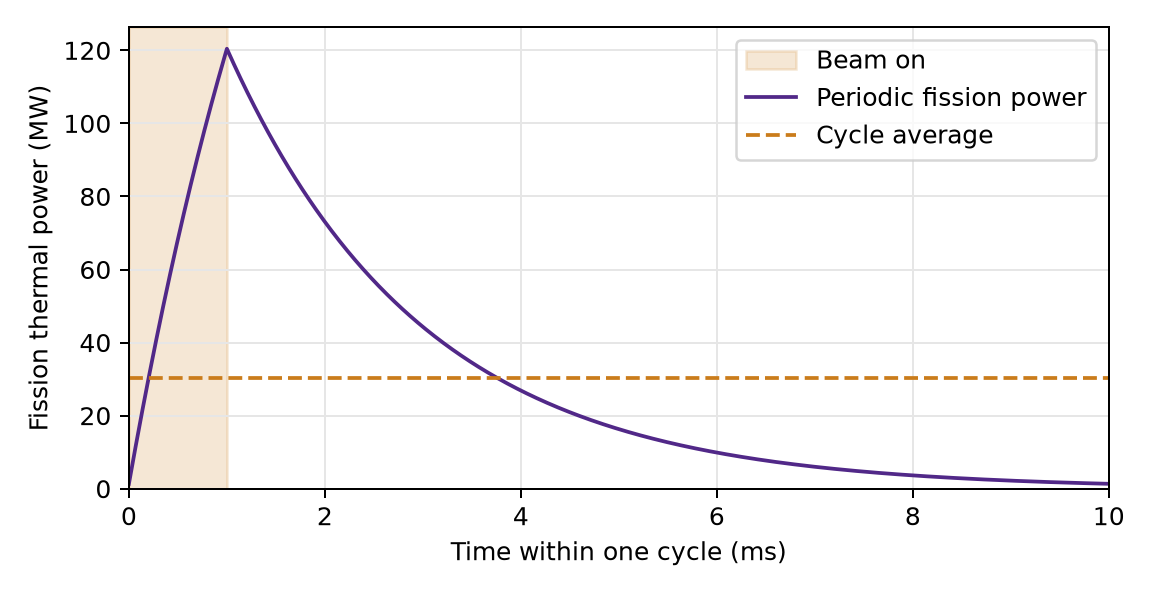
\includegraphics[width=.86\linewidth]{hw26_pulse_power.png}
\end{center}
\end{draftsolution}
